\themaM
\graphicspath{{../Ch26_Volumes_et_capacites/Images/}}

\chapter{Volume du cube\\et du pavé}
\label{C30}

%%%%%%%%%%%%%%%%%%%%%%%%%%%%%%%%%%%%%%%%%%
\begin{prerequis}[Connaissances et compétences abordées]
   \begin{itemize}
      \item Déterminer le volume d’un pavé en utilisant une formule : formules du volume d’un cube, d’un pavé droit.
   \end{itemize}
\end{prerequis}

\vfill

\begin{debat}[Débat : le Rubik's cube]
   Le Rubik's {\bf cube} est un casse-tête inventé par l'architecte hongrois {\it Ernö Rubik} en 1974. Il prend la forme d'un cube, traditionnellement à 3 petits cubes de côté, soit 36 faces et 27 petits cubes (mais il existe de très nombreuses versions allant jusqu'à 10 petits cubes de côté ou avec des formes différentes). De nombreux concours sont organisés chaque année pour le résoudre, le record actuel est de 3,47 secondes !!!
   \begin{center} 
      \begin{pspicture}(-2,-1.8)(2,2.3)
         \psSolid[viewpoint=20 30 10,a=2,object=cube,ngrid=3,fcol=0 (yellow) 1 (yellow) 2 (yellow) 3 (yellow) 4 (yellow) 5 (yellow) 6 (yellow) 7 (yellow) 8 (yellow) 9 (red) 10 (red) 11 (red) 12 (red) 13 (red) 14 (red) 15 (red) 16 (red) 17 (red) 36 (blue) 37 (blue) 38 (blue) 39 (blue) 40 (blue) 41 (blue) 42 (blue) 43 (blue) 44 (blue) ]
      \end{pspicture}
   \end{center}
   \bigskip
   \begin{cadre}[B2][F4]
      \begin{center}
         Vidéo : \href{https://www.youtube.com/watch?v=cyDmtUDBYzY}{\bf Comment le Rubik’s Cube est devenu culte}, chaîne YouTube {\it Le Monde}.
      \end{center}
   \end{cadre}
\end{debat}

\vfill

\textcolor{PartieGeometrie}{\sffamily\bfseries Cahier de compétences} : chapitre 12, exercices 13 ; 14 ; 18 ; 19 ; 25 à 32.


%%%%%%%%%%%%%%%%%%%%%%%%%%%%%%%%%%%%
%%%%%%%%%%%%%%%%%%%%%%%%%%%%%%%%%%%%
\activites

\begin{activite}[Des petits cubes]
   {\bf Objectifs :} déterminer le volume d'un cube et d'un pavé droit par dénombrement ; analyser un solide en trois dimensions.
   \begin{QCM}
      \partie[volume d'un pavé]
         On considère la pavé droit suivant : \quad \para{} composé de petits cubes identiques \quad \psline(0,0.5)(0,0)(0.5,0)(0.5,0.5)(0,0.5)(0.25,0.75)(0.75,0.75)(0.75,0.25)(0.5,0) \psline(0.5,0.5)(0.75,0.75) \\ [5mm]
         \begin{tabular}{C{5}|C{5}|C{5}}
            Colorier la \og tranche \fg{} de devant de ce pavé droit
            &
            Colorier la \og tranche \fg{} du dessus de ce pavé droit
            &
            Colorier la \og tranche \fg{} de côté de ce pavé droit \\ [3mm]
            \para{}     
            &
            \para{}
            &
            \para{} \\
            Combien de petits cubes possède cette tranche ?
            &
            Combien de petits cubes possède cette tranche ?
            &
            Combien de petits cubes possède cette tranche ? \\ [1mm]
            \pf & \pf & \pf \\ [3mm]
            Combien de fois cette tranche apparait-elle dans ce pavé droit ?
            &
            Combien de fois cette tranche apparait-elle dans ce pavé droit ?
            &
            Combien de fois cette tranche apparait-elle dans ce pavé droit ? \\ [1mm]
            \pf & \pf & \pf \\ [3mm]
            En déduire le nombre de petits cubes dans ce pavé droit.
            &
            En déduire le nombre de petits cubes dans ce pavé droit.
            &
            En déduire le nombre de petits cubes dans ce pavé droit. \\ [1mm]
            \pf & \pf & \pf \\ [3mm]
         \end{tabular}
   \bigskip
   \partie[volume d'un cube]
      Colorier dans ce pavé un cube de plus grande taille possible : \para{} \\ [3mm]
      Combien y a-t-il de petits cubes dans ce cube ? \pf \\
   \end{QCM}
\end{activite}


%%%%%%%%%%%%%%%%%%%%%%%%%%%%%%
%%%%%%%%%%%%%%%%%%%%%%%%%%%%%%
\cours 

\section{Volumes d'un pavé} %%%%%%%%%%

\begin{propriete}
   Le volume d'un pavé droit, ou d'un parallélépipède rectangle de dimensions $L, \ell$ et $h$ vaut :
   $${\cal V}=L\times \ell\times h$$
\end{propriete}

\begin{center}
   \begin{pspicture}(-0.5,-0.7)(5,3.5)
      \pspolygon(0,0)(3,0)(4,1)(4,3)(1,3)(0,2)
      \psline(0,2)(3,2)(3,0)
      \psline(3,2)(4,3)
      \psline[linestyle=dashed](0,0)(1,1)(4,1)
      \psline[linestyle=dashed](1,1)(1,3)
      \psset{linecolor=B1}
      \psline{<->}(0,-0.3)(3,-0.3)
      \rput(1.5,-0.6){\textcolor{B1}{$L$}}
      \psline{<->}(-0.3,0)(-0.3,2)
      \rput(-0.6,1){\textcolor{B1}{$h$}}
      \psline{<->}(-0.2,2.2)(0.9,3.3)
      \rput(0.2,3){\textcolor{B1}{$\ell$}}
   \end{pspicture}
\end{center}

\begin{remarque}
   dans la formule, il faut que toutes les dimensions soient exprimées dans la même unité $u$, l'unité de volume sera alors $u^3$.
\end{remarque}

\begin{exemple}
   Une piscine a pour dimensions \um{9} de long, \um{5} de large et \ucm{150} de hauteur. \\
   Quel est son volume en \umc{} ? \\
   Quelle est sa capacité en \ul{} ?
   \correction
      $\mathcal{V} =\um{9}\times\um{5}\times\um{1,5} =\umc{67,5}$. \\
      Pour déterminer sa capacité en \ul{}, il faut convertir des \umc{} en \udmc{} puis utiliser la relation $\udmc{1} =\ul{1}$ : \\
      $\umc{67,5} =\udmc{67500} =\ul{67500}$.
\end{exemple}


\section{Volume d'un cube} %%%%%%%%%%

\begin{propriete}
   Le volume d'un cube de côté $c$ vaut : ${\cal V}=c\times c\times c =c^3$.
\end{propriete}

\begin{center}
   \begin{pspicture}(-0.5,-0.5)(5,3.5)
      \pspolygon(0,0)(2,0)(3,1)(3,3)(1,3)(0,2)
      \psline(0,2)(2,2)(2,0)
      \psline(2,2)(3,3)
      \psline[linestyle=dashed](0,0)(1,1)(3,1)
      \psline[linestyle=dashed](1,1)(1,3)
      \psset{linecolor=B1}
      \psline{<->}(0,-0.3)(2,-0.3)
      \rput(1,-0.6){\textcolor{B1}{$c$}}
      \psline{<->}(-0.3,0)(-0.3,2)
      \rput(-0.6,1){\textcolor{B1}{$c$}}
      \psline{<->}(-0.2,2.2)(0.9,3.3)
      \rput(0.2,3){\textcolor{B1}{$c$}}
   \end{pspicture}
\end{center}

\begin{remarque}
   le volume du cube est un cas particulier du volume du pavé avec $L =\ell =h =c$.
\end{remarque}

\begin{exemple}
   Un Rubik's Cube a pour côté 5,5 cm. \\
   Quel est son volume en \ucmc{} ?
   \correction
      $\mathcal{V} =\ucm{5,5}\times\ucm{5,5}\times\ucm{5,5} = \ucmc{166,375}$.
\end{exemple}

%%%%%%%%%%%%%%%%%%%%%%%%%%%%%%%%%%%%%%
\exercicesbase

\begin{colonne*exercice}

\serie{Calcul de volumes} %%%%%

\begin{exercice} %1
   Une boîte a la forme d'un pavé droit de dimensions \ucm{12}, \ucm{8} et \ucm{5}.
   \begin{center}
      \begin{pspicture}(0,0.25)(3.6,3)
         \pspolygon(0,0)(3,0)(3.6,0.6)(3.6,2.6)(0.6,2.6)(0,2)
         \psline(0,2)(3,2)(3,0)
         \psline(3,2)(3.6,2.6)
         \psline(0,1.6)(3,1.6)(3.6,2.2)
         \psline(2.25,0)(2.25,0.25)(3,0.25)(3.25,0.5)(3.25,0.25)
         \psline(2.5,0)(2.5,0.25)
         \psline(2.75,0)(2.75,0.5)(3,0.5)(3.125,0.625)(3.125,0.125)
      \end{pspicture}
   \end{center}
   \begin{enumerate}
      \item Calculer le nombre de cubes de côté \ucm{1} que l'on peut ranger dans cette boîte.
      \item Déterminer le nombre de cubes de côté \umm{1} que l'on peut ranger dans cette boîte.
      \item Exprimer son volume en \ucmc{} puis en \ummc{}.
   \end{enumerate}
\end{exercice}

\begin{exercice} %2
   Calculer le volume :
   \begin{enumerate}
      \item d'un pavé droit possédant deux faces opposées carrées de côté \ucm{5} et une hauteur de \ucm{7}.
      \item d'un cube de côté \udm{2,5}.
      \item d'un pavé droit dont la hauteur est de \ucm{9}, la largeur mesure la moitié de la hauteur et la longueur est le triple de la hauteur.
   \end{enumerate}
\end{exercice}

\medskip

\begin{exercice} %3
   Pour transporter des marchandises par bateau ou camion, on utilise des containers dont la longueur est de \um{12}, la largeur de \um{2,5} et la hauteur de \um{2,5}.
   \begin{enumerate}
       \item Calculer le volume d'un container en mètre cube.
       \item Exprimer ses dimensions en décimètre.
       \item Donner son volume en décimètre cube.
   \end{enumerate}
\end{exercice}

\medskip

\begin{exercice} %4
   Un réservoir de chasse d'eau a la forme d'un pavé droit de \ucm{30} de longueur, \ucm{24} de largeur et \ucm{18} de hauteur. \\
   Il est rempli aux trois quarts de sa hauteur. \\
   Combien de litres d'eau sont utilisés lorsqu'on tire cette chasse d'eau ?
\end{exercice}

\medskip

\begin{exercice} %5
   La fiche technique d'un congélateur donne les dimensions intérieures suivantes :
   \begin{center}
      \fbox{(L $\times$ P $\times$ H) en cm : 44 $\times$ 42 $\times$47}
   \end{center}
   Déterminer la capacité de ce congélateur en litres.
\end{exercice}

\columnbreak

\begin{exercice} %6
   Classer ces pavés du plus petit au plus grand volume en expliquant.
   \begin{center}
      {\psset{unit=0.8,fillstyle=solid,fillcolor=A2}
      \small
      \begin{pspicture}(1,0)(10,10)
         \pspolygon(1,1)(5,1)(6,2)(6,3.5)(2,3.55)(1,2.5)
         \psline(1,2.5)(5,2.5)(6,3.5)
         \psline(5,2.5)(5,1)
         \rput(3,0.6){\ucm{4}}
         \rput{90}(0.6,1.75){\ucm{1,5}}
         \rput{45}(5.8,1.2){\ucm{2,5}}
         \pspolygon(1,5)(3.5,5)(4.5,6)(4.5,8.5)(2,8.5)(1,7.5)
         \psline(1,7.5)(3.5,7.5)(4.5,8.5)
         \psline(3.5,7.5)(3.5,5)
         \rput(2.25,4.6){\ucm{2,5}}
         \rput(2.25,6.25){\white cube}
         \pspolygon(8,2)(9,2)(9.9,2.9)(9.9,9.9)(8.9,9.9)(8,9)
         \psline(9,2)(9,9)(9.9,9.9)
         \psline(9,9)(8,9)
         \rput(8.5,1.6){\ucm{1}}
         \rput{45}(9.7,2.1){\ucm{2,2}}
         \rput{90}(7.6,5.5){\ucm{7}}
      \end{pspicture}}
   \end{center}
\end{exercice}


\serie{Défis} %%%%%

\begin{exercice} %7
   Comment pourrait-on calculer le volume de ces deux pièces de jeu ?
   \begin{center}
      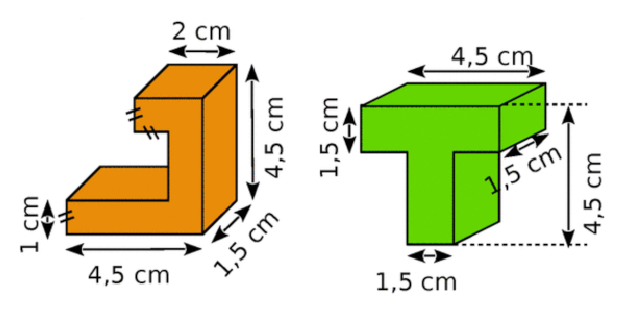
\includegraphics[width=8cm]{pieces}
   \end{center}
\end{exercice}

\bigskip

\begin{exercice} %8
   Un bac à fleurs est réalisé en bois à l'aide de planches de \umm{12} d'épaisseur. La largeur du bac est de \ucm{110}, sa longueur de \ucm{65} et sa hauteur de \ucm{45} (ces dimensions sont mesurées à l'extérieur). \\
   Combien de sacs de terre de \ul{25} faut-il acheter pour remplir le bac  ?
\end{exercice}

\vfill\hfill{\it\footnotesize Source : D’après Les cahiers Sésamath 6e. Magnard-Sesamath 2017}

\end{colonne*exercice}


%%%%%%%%%%%%%%%%%%%%%
%%%%%%%%%%%%%%%%%%%%%
\Recreation

\begin{activite}[Des pavés de toutes sortes]
   {\bf Objectifs :} calculer le volume d'un pavé ; différencier volume et capacité ; résoudre un problème dans le domaine des grandeurs et mesures. \\

      \partie[observations]
         Quelle action est matérialisée par le schéma suivant ? \\ [2mm]
         \pf \\ [2mm]
         \pf \\
         \begin{center}
            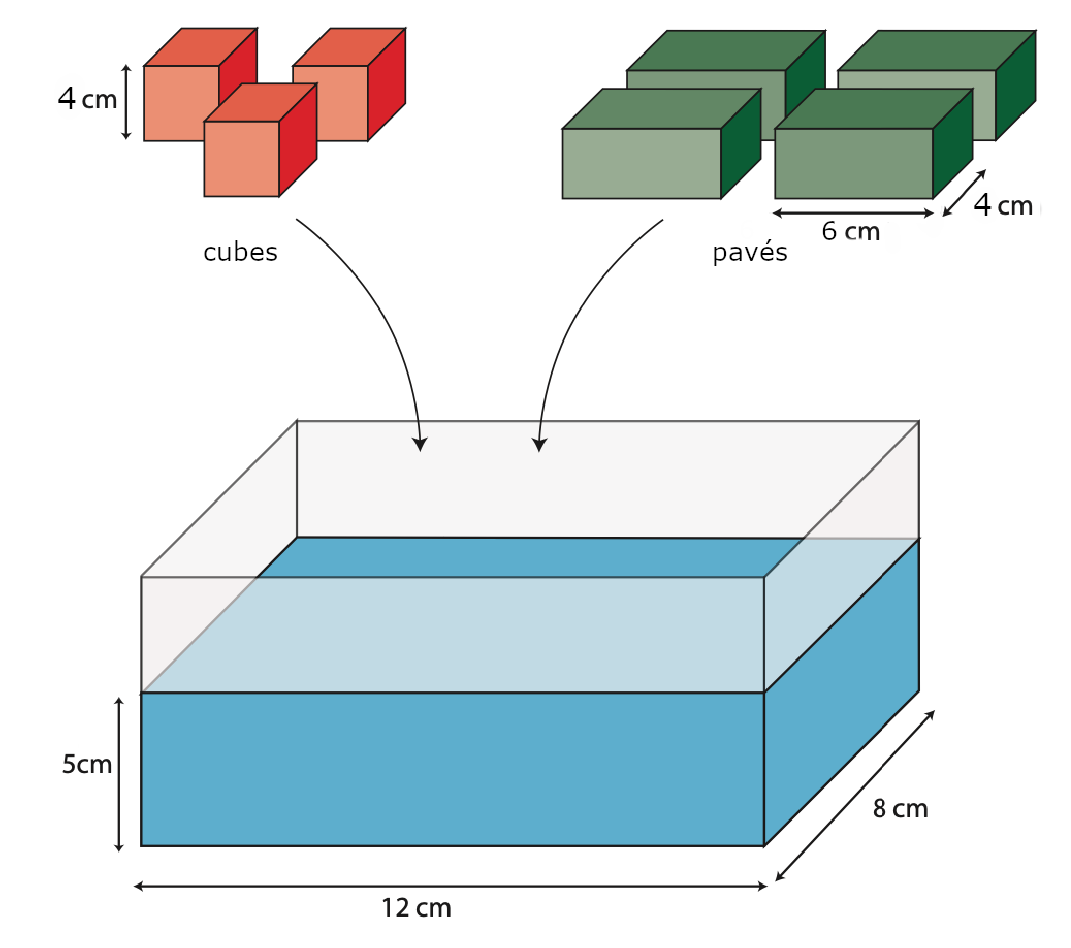
\includegraphics[width=9cm]{piscine}
         \end{center}
      \partie[questions]
         \begin{enumerate}
            \item Quel est le volume d'eau en \ucmc{} contenu dans la boite transparente ? \\ [3mm]
               \pf \\
            \item Quelle est la capacité d'eau en L contenue dans la boite transparente ? \\ [3mm]
               \pf \\
            \item Dans la bassine, on plonge trois cubes et quatre pavés. Quelle doit être la hauteur des pavés pour que l'eau monte de \ucm{4} ? \\ [2mm]
               \pf \\ [3mm]
               \pf \\ [3mm]
               \pf
         \end{enumerate}

      \vfill \hfill {\it\footnotesize Source : d'après l'activité \href{http://www-irem.univ-paris13.fr/site_spip/IMG/pdf/des_paves_dans_la_mare_2_noir.pdf}{Des pavés dans la mare}, IREM Paris Nord.}
\end{activite}

